\section{Signal model detector response table}

In this appendix we describe digital tables which can be used to construct an accurate signal model for this analysis given any input recoil spectrum $\mathrm{d}R/\mathrm{d}E$. A visualisation of the tables is shown in Fig. \ref{fig:smeartable_highE}, and in section \ref{app:example_code} we show a simple example of how to use the supplied tables in Python. Currently we provide these tables only for the high E analysis region.

The signal model for the high E analysis region can be expressed analytically in the form:
%
\begin{align}
\label{eq:high2D}
  \frac{\mathrm{d} R}{\mathrm{d}\cSi} &= \int \! \frac{\mathrm{d}R}{\mathrm{d}E}.\epsilon_\mathrm{S1}(\cSi) .\epsilon_\mathrm{S2'}(E).p_\mathrm{S1}(\mathrm{\cSi}|E) \, \mathrm{d}E \\
  &= \int \! \frac{\mathrm{d}R}{\mathrm{d}E} G(\cSi,E) \, \mathrm{d}E
\end{align}
%
where $\epsilon_\mathrm{S1}(\cSi)$ and $\epsilon_\mathrm{S2'}(E)$ represent analysis cut efficiencies, $p_\mathrm{S1}(\mathrm{\cSi}|E)$ encodes detector effects, and $\mathrm{d}R/\mathrm{d}E$ gives the theoretically predicted nuclear recoil rate from WIMP scattering. In the second line we emphasise that all the detector and analysis effects can be encoded in a single function $G(\cSi,E)$. To make a signal prediction for the bins in our analysis this expression needs to be integrated over the appropriate range of $\cSi$ for each bin (and divided by two to account for the banding structure in $\cSiib$):
%
\begin{equation}
  R_\mathrm{bin_i} = \frac{1}{2}\int_{\mathrm{lower}_i}^{\mathrm{upper}_i} \! \frac{\mathrm{d} R}{\mathrm{d}\cSi} \, \mathrm{d}\cSi
\end{equation}
%
With some simple rearrangement this rate can be written in terms of an integral over the detector response function $G$ as follows
%
\begin{align}
  R_\mathrm{bin_i} &= \frac{1}{2}\int\frac{\mathrm{d} R}{\mathrm{d}E}\int_{\mathrm{lower}_i}^{\mathrm{upper}_i} \! G(\cSi,E) \, \mathrm{d}\cSi \, \mathrm{d}E \\
 &= \int\frac{\mathrm{d} R}{\mathrm{d}E} G'_i(E) \mathrm{d}E
\end{align}
%
where in the last line we absorb the factor of $1/2$ into the definition of $G'_i$. We see here that the signal rate for each bin can be expressed as an integral over the recoil spectrum times a detector response function $G'_i$ for that bin. It is these detector response functions which are shown in Fig. \ref{fig:smeartable_highE}, and which we provide digitally for use by the community. With these tables it is simple to produce a signal model for our analysis for any input theoretical recoil spectrum. The functions $G'_i$ are provided for three values of the nuisance variable $\Leff$, namely the median value and values at $\pm 1 \sigma$ in $\Leff$. From these, along with the measured background rates given in table \ref{table:BinDef}, one may construct a likelihood which accounts for uncertanities in $\Leff$, however simply using the $-1\sigma$ value produces quite an accurate prediction and is generally conservative.

Details of how to extract and use the provided $G'$ functions are given in the example of section \ref{app:example_code}. 

\begin{figure}
\centerline{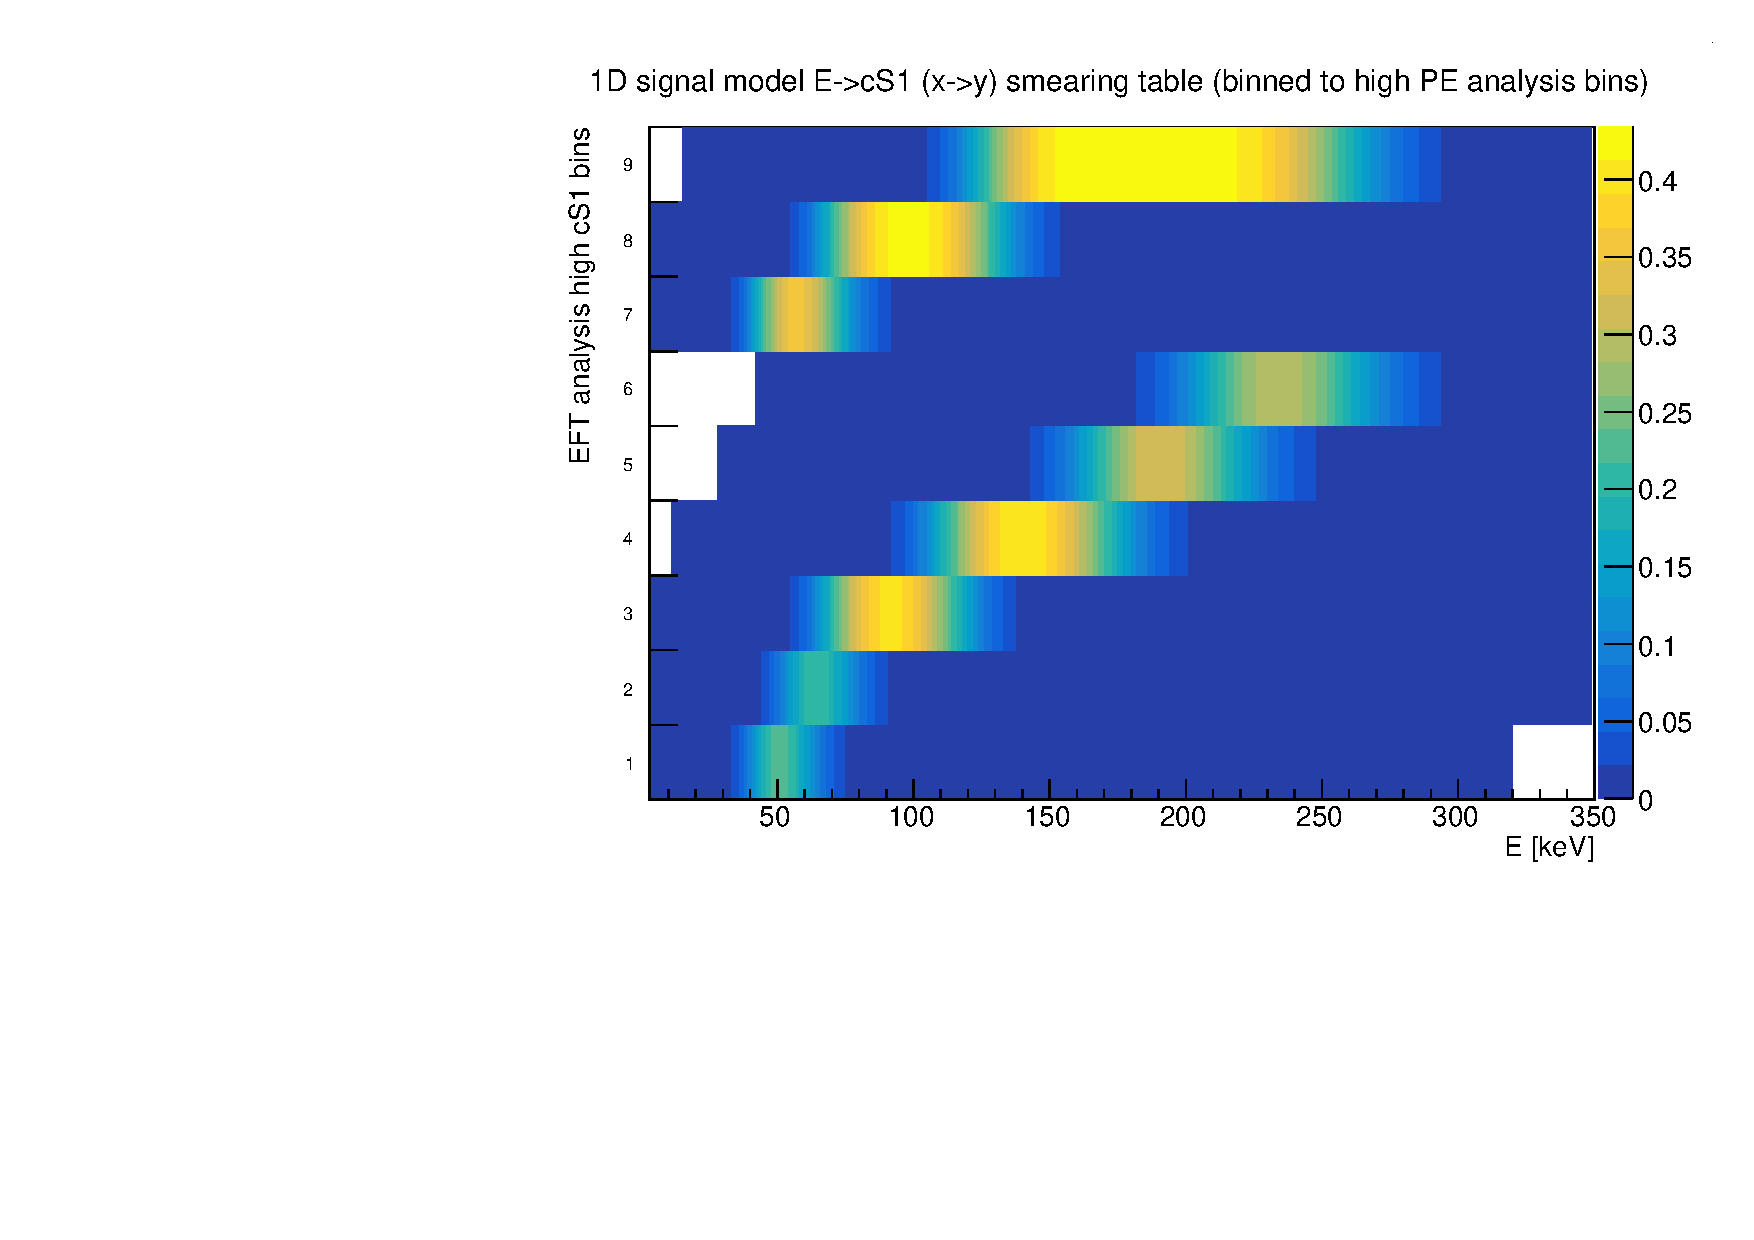
\includegraphics[width=1.\linewidth]{Figures/smeartable_highE}}
\caption{A visualisation of the detector response table for $-1\sigma$ (i.e. conservative) $\Leff$, as provided in the supplementary material. The table visualisation shows, on the y axis, the bins used for the high E signal region of this analysis. The $x$ axis shows recoil energies, and the colours give the probability density for a recoil of a given recoil energy to produce an event in each analysis bin. To produce a signal model for this analysis, one simply multiplies the table values by $\mathrm{d}R/\mathrm{d}E$ and integrates over $E$. The result is the predicted signal rate for each analysis bin.}
\label{fig:smeartable_highE}
\end{figure}  

\subsection{Example code}
\label{app:example_code}
\begin{lstlisting}
import ROOT
import h5py
import numpy as np
from scipy.interpolate import interp1d

# Test dR/dE
drde_dir = "/home/farmer/repos/EFTtools/recoil_spectrum_tables/XeComb"
fnamehigh = "{0}/IDM_XeComb_NR_highE_c6p=c6n.h5".format(drde_dir)
f_dRdE_high = h5py.File(fnamehigh,'r')
dath = f_dRdE_high["delm0"][:].T
Erh, dRdEh = dath[0], dath[17] # first column is El, rest contain dRdE for each mass (1 TeV selected)
# Rate is for coupling squared of 1; let us rescale it to a value near the limit (1e3)
# Also have to correct the exposure from benchmark
# value of 7800 kg.days
dRdEh = dRdEh * (1e3/1.) * 224.6*34. / 7800.

# Smearing table root file
datadir = "recorded_results/fixed_Er3keV_cut_LE+HE_smeartable2"
fsmear = "{0}/SmearTables.root".format(datadir)

def get_table(rootfile,objname):
    """Extract 2D ROOT histogram from file""" 
    f = ROOT.TFile(rootfile, 'r')
    h = f.Get(objname)
    h.SetDirectory(0)
    Nx = h.GetNbinsX()
    Ny = h.GetNbinsY()
    # Get arrays of bin edges
    x = np.array([h.GetXaxis().GetBinLowEdge(i+1) for i in range(Nx+1)])
    y = np.array([h.GetYaxis().GetBinLowEdge(j+1) for j in range(Ny+1)])
    Z = np.zeros((Nx,Ny))
    for i in range(Nx):
        for j in range(Ny):
            Z[i,j] = h.GetBinContent(i+1,j+1)
    return x, y, Z

def TrapI(x,y):
    """Simple trapezoid integration"""
    w = x[1:] - x[:-1]
    h = (y[1:] + y[:-1])/2.
    return np.sum(w*h,axis=0)

def get_signal_model(Er,dRdE,G,E):
    """Function for computing a signal model based on 2D smearing tables.
    Need to align dRdE samples with Gl samples, or vice-versa, in order to do the integration
    Easiest to interpolate the dRdE onto the Gl samples I think.
    Er, dRdE - theoretical recoil spectrum
    G - smearing table to use
    E - sampled recoil energy values in G"""
    f_dRdE = interp1d(Er,dRdE,bounds_error=False,fill_value=0) # assume spectrum is zero outside supplied data range
    dRdE_matched = f_dRdE(E)
    dRdcS1 = TrapI(E[:,np.newaxis],G*dRdE_matched[:,np.newaxis])
    return dRdcS1

# Note; pdf values in bins are associated with the LOWER bin edge value
Eh, cS1h, Gh = get_table(fsmear,"th2f_Leff-1.0000_highSR_binned")
dR_htab = get_signal_model(Erh,dRdEh,Gh,Eh[:-1]) 

for i,R in enumerate(dR_htab):
  print "bin {0}: rate = {1:.2g}".format(i+1,R)
\end{lstlisting}

Output:

\begin{lstlisting}
bin 1: rate = 0.081
bin 2: rate = 0.098
bin 3: rate = 0.35
bin 4: rate = 0.46
bin 5: rate = 0.29
bin 6: rate = 0.22
bin 7: rate = 0.18
bin 8: rate = 0.47
bin 9: rate = 0.84
\end{lstlisting}
